\section{Business Intelligence vs. Business Analytics: ¿Cuál es la diferencia?} 
\textbf{Elegir entre Business Intelligence y Business Analytics}
\vspace{5mm} %5mm vertical space

Las organizaciones están empezando a ver que los datos y el contenido no deben considerarse aspectos separados de la gestión de la información, sino que deben gestionarse en un enfoque empresarial integrado. Muchas empresas se están moviendo hacia la inteligencia comercial operativa, que actualmente no cuenta con los proveedores adecuados.\\

\vspace{5mm} %5mm vertical space
\begin{center}
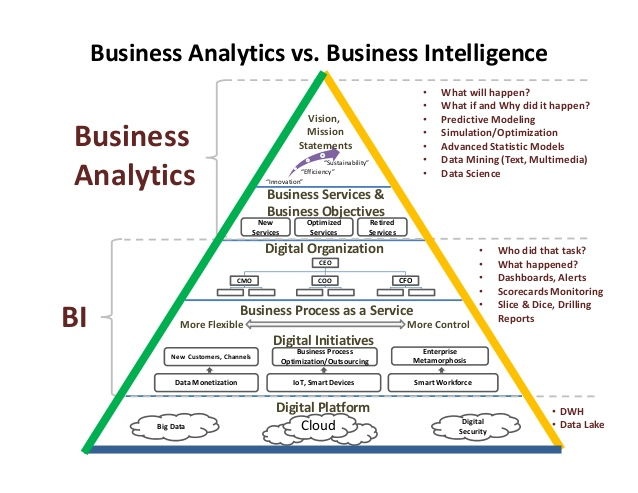
\includegraphics[width=14cm]{./Imagenes/003}
\end{center}	
\vspace{12mm} %5mm vertical space

\textbf{Evalúa tus necesidades} Tradicionalmente, los proveedores de inteligencia empresarial se enfocaban principalmente en las empresas, pero ahora hay un cambio de paradigma de que BI se mude a las pequeñas y medianas empresas. El autoservicio de BI es un enfoque principal de estas compañías más pequeñas.

La inteligencia empresarial de autoservicio (SSBI) es un enfoque para el análisis de datos que permite a los usuarios acceder y trabajar con datos corporativos aunque no tengan experiencia en análisis o ciencia de datos. Por lo general, cuenta con una interfaz de usuario más amigable y no implica codificación, por lo que su joe regular puede operarlo.\\


\textbf{Elija con Intención} Elegir la solución para su negocio depende de sus intenciones. Si está satisfecho con su modelo de negocio en general y desea principalmente mejorar las operaciones, aumentar la eficiencia y cumplir los objetivos de la organización, la inteligencia empresarial puede ser una solución óptima. En particular, las empresas que confían en los informes en tiempo real tienden a inclinarse hacia 
BI, ya que están preocupados por lo que pueden mejorar aquí y ahora.

Por otro lado, si tiene la intención de cambiar los procesos de su empresa, o incluso su modelo de negocio completo, pero todavía no tiene los conocimientos necesarios, el análisis de negocios podría ser la mejor opción.

Las empresas que requieren una gran cantidad de datos (por ejemplo, la necesidad de almacenamiento de datos) e informes intuitivos deben considerar seriamente la inteligencia empresarial. BI tiene las ventajas adicionales de dirigirse a las áreas débiles de una empresa y proporcionar información accionable sobre esos problemas. Las herramientas de inteligencia comercial son excelentes soluciones para los gerentes que desean mejorar la toma de decisiones y comprender la productividad, los procesos de trabajo y los empleados de su organización. Luego, con esa comprensión, mejore su negocio desde cero.

